
%% This work may be distributed and/or modified under the conditions of the LaTeX Project Public License, either version 1.3 of this license or (at your option) any later version. The latest version of this license is in http://www.latex-project.org/lppl.txt and version 1.3 or later is part of all distributions of LaTeX version 2005/12/01 or later. This work has the LPPL maintenance status `maintained'. Further information about abnTeX2 are available on https://github.com/abntex/abntex2 | https://www.abntex.net.br/
%%
%% The Current maintainer of this template is Geraldo Pereira de M. Jr. 
%% Contact: geraldo.pmj@gmail.com
%%
\documentclass[
	12pt,				% tamanho da fonte
	oneside,			% impressão em um lado da folha (relatório entregue em PDF)
	a4paper,			% tamanho do papel.
	sumario = tradicional,
	% -- opções da classe abntex2 --
	%chapter=TITLE,		% títulos de capítulos convertidos em letras maiúsculas
	%section=TITLE,		% títulos de seções convertidos em letras maiúsculas
	%subsection=TITLE,	% títulos de subseções convertidos em letras maiúsculas
	%subsubsection=TITLE,% títulos de subsubseções convertidos em letras maiúsculas
	% -- opções do pacote babel --
	english,			% idioma adicional para hifenização
	brazilian			% o último idioma é o principal do documento
	]{abntex2}
% ---
% Pacotes básicos 
% --
\usepackage{times} %{lmodern}	% Usa a fonte Latin Modern			
\usepackage[T1]{fontenc}% Selecao de codigos de fonte.
\usepackage[utf8]{inputenc}% Codificacao do documento (conversão automática dos acentos)
\usepackage{indentfirst}	% Indenta o primeiro parágrafo de cada seção.
\usepackage[top=30mm, bottom=20mm, left=30mm, right=20mm]{geometry}
\usepackage{color}		% Controle das cores
\usepackage{graphicx}	% Inclusão de gráficos
\graphicspath{ {./figuras/} }
\usepackage{microtype} 	% para melhorias de justificação
\usepackage{fancyhdr} %define o estilo do documento
\usepackage{array} %permite o uso de tabelas
\usepackage{longtable} %permite o uso de tabelas personalizadas
\usepackage{rotating} %permite rotacionar imagens
\usepackage{tikz} %permite o desenho de formas geométricas simples dadas suas características
\usepackage{PPGAN}
\usepackage{ragged2e}
\usepackage{csquotes}
\usepackage{pdfpages}
\usepackage{amsmath}
\usepackage{amssymb}
% ---
% Pacotes de citações
% ---
\usepackage[style=abnt, repeatfields, backend=biber]{biblatex}
\addbibresource{referencias.bib} % Seus arquivos de

\ifthenelse{\equal{\ABNTEXisarticle}{true}}{%
\renewcommand{\maketitlehookb}{}
}{}
\PassOptionsToPackage{brazilian,english}{babel}

\DeclareUnicodeCharacter{031C}{ç}


% ---
% Configurações de aparência do PDF final

% alterando o aspecto da cor azul
\definecolor{blue}{RGB}{41,5,195}

% informações do PDF
\makeatletter
\hypersetup{
     	%pagebackref=true,
		pdftitle={\@title}, 
		pdfauthor={\@author},
    	pdfsubject={\imprimirpreambulo},
	    pdfcreator={\@author},
		pdfkeywords={palavra-chave}{palavra-chave}{palavra-chave}, 
		colorlinks=true,       		% false: boxed links; true: colored links
    	linkcolor=black,          	% color of internal links
    	citecolor=black,        		% color of links to bibliography
    	filecolor=magenta,      		% color of file links
		urlcolor=black,
		bookmarksdepth=4}
\makeatother
% --- 

% ---
% Posiciona figuras e tabelas no topo da página quando adicionadas sozinhas
% em um página em branco. Ver https://github.com/abntex/abntex2/issues/170
\makeatletter
\setlength{\@fptop}{5pt} % Set distance from top of page to first float
\makeatother
% ---

% ---
% Possibilita criação de Quadros e Lista de quadros.
% Ver https://github.com/abntex/abntex2/issues/176
%
\newcommand{\quadroname}{Quadro}
\newcommand{\listofquadrosname}{Lista de quadros}

\newfloat[chapter]{quadro}{loq}{\quadroname}
\newlistof{listofquadros}{loq}{\listofquadrosname}
\newlistentry{quadro}{loq}{0}

% configurações para atender às regras da ABNT
\setfloatadjustment{quadro}{\centering}
\counterwithout{quadro}{chapter}
\renewcommand{\cftquadroname}{\quadroname\space} 
\renewcommand*{\cftquadroaftersnum}{\hfill--\hfill}

\setfloatlocations{quadro}{hbtp} % Ver https://github.com/abntex/abntex2/issues/176
% ---

% --- 
% Espaçamentos entre linhas e parágrafos 
% --- 

% O tamanho do parágrafo é dado por:
\setlength{\parindent}{1.2cm}
% Controle do espaçamento entre um parágrafo e outro:
\setlength{\parskip}{0.3cm}  % tente também \onelineskip
\linespread{1.7}
\renewcommand{\baselinestretch}{1.5}
%\DeclareUnicodeCharacter{0301}{i}

\setlength\bibitemsep{4\itemsep}


\usetikzlibrary{calc,arrows.meta}

% ---------------------------------------------------------------
% Código VHDL no estilo dos slides (palavras reservadas em azul,
% comentários em verde, fundo amarelo-claro)
% ---------------------------------------------------------------
\usepackage{xcolor}
\usepackage{listings}
\definecolor{kwblue}{RGB}{0,105,190}
\definecolor{cmtgreen}{RGB}{0,150,80}
\definecolor{codebg}{RGB}{255,248,215}
\definecolor{codeborder}{RGB}{210,160,0}
\lstdefinelanguage{VHDL}{
  sensitive=false,
  morecomment=[l]{--}
}
\lstdefinestyle{vhdl}{
  language=VHDL,
  morekeywords=[1]{ENTITY,ARCHITECTURE,LIBRARY,USE,PORT,IS,OF,BEGIN,END,
    SIGNAL,CONSTANT,VARIABLE,WITH,SELECT,WHEN,ELSE,OTHERS,IN,OUT,
    BUFFER,INOUT,DOWNTO,TO,RANGE,AND,OR,XOR,NOT,NAND,NOR,XNOR,ALL,
    entity,architecture,library,use,port,is,of,begin,end,signal,constant,
    variable,with,select,when,else,others,in,out,buffer,inout,downto,to,
    range,and,or,xor,not,nand,nor,xnor,all},
  morekeywords=[2]{STD_LOGIC,STD_LOGIC_VECTOR,STD_ULOGIC,INTEGER,BIT,
    BIT_VECTOR,UNSIGNED,SIGNED,NATURAL,POSITIVE,BOOLEAN,
    std_logic,std_logic_vector,std_ulogic,integer,bit,bit_vector,unsigned,
    signed,natural,positive,boolean},
  keywordstyle=[1]\color{kwblue}\bfseries,
  keywordstyle=[2]\color{kwblue}\bfseries,
  commentstyle=\color{cmtgreen}\itshape,
  stringstyle=\color{black},
  basicstyle=\ttfamily\footnotesize,
  backgroundcolor=\color{codebg},
  frame=single, rulecolor=\color{codeborder},
  framesep=4pt, xleftmargin=4pt, xrightmargin=4pt,
  aboveskip=6pt, belowskip=2pt,
  breaklines=true, breakatwhitespace=true,
  showstringspaces=false, columns=fullflexible,
  keepspaces=true, tabsize=4, upquote=true,
  numbers=left,
  numberstyle=\tiny,
}
\lstset{style=vhdl}

% ---
% Pacote que deixa vários comandos do LaTex comumente usados em português. Pode ver exemplos na Introdução. Contudo pode continuar a usar os comandos do LaTex normalmente se preferir.
% ---
\usepackage{PTLatexCommands}

% ---
% Informações de dados para CAPA e FOLHA DE ROSTO
% ---
\titulo{Desenvolvimento de uma Unidade Lógica e Aritmética (ALU) de 8 Bits em VHDL Concorrente}
\autor{Ariel Inácio Jordão Coelho\break Lucca Mendes Alves Pellegrini} % TODO: substituir pelo seu nome
\local{Belo Horizonte}
\data{2026}
\orientador{Francisco Manoel Pinto Garcia} % TODO: substituir
\instituicao{%
  Pontifícia Universidade Católica de Minas Gerais
  \par
  Engenharia de Computação}
\tipotrabalho{Relatório Técnico (Graduação)}
% O preambulo deve conter o tipo do trabalho, o objetivo, 
% o nome da instituição e a área de concentração 
\preambulo{Relatório técnico do Primeiro Trabalho Pratico (TP1), apresentado à
disciplina de Sistemas Reconfiguráveis do Curso de
Engenharia de Computação da Pontifícia Universidade Católica de Minas Gerais.\linebreak
\textbf{Área de concentração}: Sistemas Digitais e Reconfiguráveis \newline
\textbf{Professor}: \imprimirorientador}

% ---
% compila o indice
% ---
\makeindex
% ---

% ----
% Início do documento
% ----
\begin{document}
\selectlanguage{brazilian}
% Retira espaço extra obsoleto entre as frases.
\frenchspacing 
%spaçamento 
%----------------------------------------------------
% ELEMENTOS PRÉ-TEXTUAIS
%----------------------------------------------------
\pretextual
%---
% Capa
%---
\imprimircapa 
%---
% Folha de rosto
% (sem ficha catalográfica neste relatório)
%---

\imprimirfolhaderosto

%---
% Inserir a ficha bibliografica
%---
% Isto é um exemplo de Ficha Catalográfica, ou ``Dados internacionais de
% catalogação-na-publicação''. Você pode utilizar este modelo como referência. 
% Porém, provavelmente a biblioteca da sua universidade lhe fornecerá um PDF
% com a ficha catalográfica definitiva após a defesa do trabalho. Quando estiver
% com o documento, salve-o como PDF no diretório do seu projeto e substitua todo
% o conteúdo de implementação deste arquivo pelo comando abaixo:
% \input{capitulos/ficha.tex}
%---
%Inserir errata
%---
%\input{capitulos/errata.tex}
%---
% Inserir folha de aprovação
%---
% \input{capitulos/aprov.tex} 
%---
% Dedicatória
%---
% \input{capitulos/dedi.tex}
%---
% RESUMOS
%---
\begin{resumo}
Este relatório apresenta o desenvolvimento de uma Unidade Lógica e Aritmética (ALU) de 8 bits, totalmente combinacional, descrita em VHDL com código exclusivamente concorrente e sintetizada no ambiente Quartus II 9.1sp2. A ALU executa 16 operações (lógicas, aritméticas, de deslocamento e de rotação) selecionadas por uma palavra de 4 bits e gera cinco flags de status: negativo, overflow, zero, half carry/borrow e carry/borrow. São descritos a especificação, a arquitetura adotada (um somador/subtrator unificado compartilhado pelas quatro operações aritméticas), o código comentado, os casos de teste e os resultados de simulação funcional, que concordam com os valores esperados.

\textbf{Palavras-chave}: ALU. VHDL. Lógica combinacional. Sistemas reconfiguráveis. Quartus.
\end{resumo}

\begin{resumo}[Abstract]
\begin{otherlanguage*}{english}
This report presents the design of an 8-bit, fully combinational Arithmetic Logic Unit (ALU) described in VHDL using concurrent code only and targeted at Quartus II 9.1sp2. The ALU performs 16 operations (logic, arithmetic, shift and rotate) chosen by a 4-bit select word and produces five status flags: negative, overflow, zero, half carry/borrow and carry/borrow. The specification, the architecture (a single adder/subtractor shared by the four arithmetic operations), the commented source code, the test cases and the functional simulation results are described; the results match the expected values.

\vspace{\onelineskip}
\noindent\textbf{Keywords}: ALU. VHDL. Combinational logic. Reconfigurable systems. Quartus.
\end{otherlanguage*}
\end{resumo}

%---
%LISTAS
%---
\pdfbookmark[0]{\listfigurename}{lof}
\listoffigures*
\cleardoublepage
\pdfbookmark[0]{\listtablename}{lot}
\listoftables*
\cleardoublepage
\begin{siglas}

  \item[ALU] \textit {Arithmetic Logic Unit} (unidade lógica e aritmética)
  \item [ASIC] \textit {Application-Specific Integrated Circuit}
  \item [EDA] \textit {Electronic Design Automation}
  \item [FPGA] \textit {Field-Programmable Gate Array}
  \item [HDL] \textit {Hardware Description Language}
  \item [IEEE] \textit {Institute of Electrical and Electronics Engineers}
  \item [LE] \textit {Logic Element}
  \item [LUT] \textit {Look-Up Table}
  \item [MSI] \textit {Medium Scale Integration}
  \item [PLD] \textit {Programmable Logic Device}
  \item [RTL] \textit {Register Transfer Level}
  \item [VHDL] \textit {VHSIC Hardware Description Language}
  \item [VHSIC] \textit {Very High Speed Integrated Circuit}

\end{siglas}
\cleardoublepage

%---
%inserir o sumario
%---
\pdfbookmark[0]{\contentsname}{toc}
\tableofcontents*
\cleardoublepage


%-----------------------------------------------------
% ELEMENTOS TEXTUAIS
%-----------------------------------------------------

\textual

%-----------------------------------------------------
%-----------------------------------------------------
\chapter{Introdução}
\label{cap:introducao}

A Unidade Lógica e Aritmética (ALU) é o bloco do processador responsável por executar as operações sobre os dados. Neste trabalho, desenvolvido na disciplina de Sistemas Reconfiguráveis, projeta-se uma ALU de 8 bits em VHDL \cite{ashenden2008,pedroni2010}, que recebe dois operandos, um carry de entrada e um código de operação, e devolve o resultado e um conjunto de flags de status.

\section{Objetivos}

O objetivo geral é descrever, simular e documentar uma ALU combinacional de 8 bits com 16 funções. Os objetivos específicos são:

\begin{itemize}
  \item descrever a ALU em VHDL usando \textbf{exclusivamente código concorrente}, com entradas e saídas dos tipos \texttt{std\_logic} e \texttt{std\_logic\_vector};
  \item garantir que o circuito seja puramente combinacional, sem \textit{latches} nem \textit{flip-flops};
  \item gerar corretamente as flags de negativo, overflow, zero, \textit{half carry/borrow} e \textit{carry/borrow};
  \item definir casos de teste, simular o projeto e comparar os resultados com os valores esperados.
\end{itemize}

\section{Ferramentas e restrições}

O projeto foi desenvolvido no Quartus II versão 9.1sp2, conforme exigido na especificação. Todo o código obedece às restrições abaixo.

\begin{itemize}
  \item Não há comandos \texttt{process}; todas as atribuições são concorrentes (\texttt{<=}, \texttt{with-select}, \texttt{when-else}).
  \item Os pacotes \texttt{std\_logic\_1164} e \texttt{numeric\_std} são usados; os tipos \texttt{unsigned} aparecem apenas como sinais internos do somador.
  \item mplementar um circuito totalmente combinacional, ou seja, sem latches nem flip-flops.
\end{itemize}

\section{Organização do relatório}

O Capítulo~\ref{cap:fundamentos} resume os conceitos necessários. O Capítulo~\ref{cap:especificacao} detalha a especificação da ALU. O Capítulo~\ref{cap:implementacao} apresenta a arquitetura e o código VHDL. O Capítulo~\ref{cap:simulacao} descreve os casos de teste e os resultados. Por fim, a Conclusão sintetiza o trabalho.

O Capítulo~\ref{cap:fundamentos} resume os conceitos de VHDL e de projeto combinacional apresentados nas aulas
e utilizados no projeto. O Capítulo~\ref{cap:especificacao} apresenta a especificação da ALU. O Capítulo~\ref{cap:implementacao} descreve a
implementação em VHDL e o Capítulo~\ref{cap:simulacao} apresenta a simulação, os casos de teste e os resultados.
Por fim, o Capítulo 6 reúne as conclusões.

%-----------------------------------------------------
\chapter{Fundamentação teórica}
\label{cap:fundamentos}

\section{Linguagens de descrição de hardware e VHDL}

Uma linguagem de descrição de hardware (HDL) é usada para a descrição formal e o projeto de
circuitos eletrônicos, sobretudo digitais. Ela permite descrever o funcionamento, a concepção
e a organização de um circuito e testá-lo por meio de simulação (GARCIA; MAGALHÃES, 2024).
Dentre as vantagens de uma HDL padronizada estão a independência do fornecedor, a porta-
bilidade e a reusabilidade. Em relação ao diagrama esquemático, a descrição por HDL oferece
projeto independente da tecnologia, facilidade de atualização, redução do tempo e do custo
de projeto e redução do volume de documentação (GARCIA; MAGALHÃES, 2024).

\secao{Estrutura de um projeto em VHDL}

Um projeto VHDL possui três unidades fundamentais \cite{aula3}:

\begin{listar}
  \item \texttt{LIBRARY}: lista os pacotes e bibliotecas usados no projeto;
  \item \texttt{ENTITY}: especifica as entradas e saídas do circuito, com o
        nome do arquivo \texttt{.vhd} igual ao nome da entidade;
  \item \texttt{ARCHITECTURE}: contém o código que descreve o funcionamento do
        circuito.
\end{listar}

Os modos das portas são \texttt{IN}, \texttt{OUT}, \texttt{BUFFER} e
\texttt{INOUT}. Uma porta \texttt{OUT} não pode ser lida dentro da
arquitetura, ao contrário de uma porta \texttt{BUFFER} \cite{aula3}. A
atribuição a um \texttt{SIGNAL} ou a uma porta usa o operador \texttt{<=}; os
comentários começam com \texttt{--} e vão até o fim da linha. A linguagem não
distingue maiúsculas de minúsculas, mas é recomendável escrever as palavras
reservadas em maiúsculas e os nomes de sinais em minúsculas \cite{aula3}.

O Código~\ref{lst:cap3ex1} reproduz o exemplo de código completo apresentado
na aula 3.

\break

\begin{lstlisting}[caption={Exemplo de ENTITY e ARCHITECTURE (aula 3).},label={lst:cap3ex1}]
ENTITY Cap3ex1 IS
    PORT (
        a     : IN BIT;
        b     : IN BIT;
        x,y,z : OUT BIT
    );
END Cap3ex1;
-----------------------------
ARCHITECTURE arch OF Cap3ex1 IS
BEGIN
    x <= a AND b;   -- saida x
    y <= a OR b;    -- saida y
    z <= a XOR b;   -- saida z
END arch;
\end{lstlisting}
\vspace{-0.3cm}
\fonte{ Codigo retirado do slide aula 6 de Garcia.}

\section{Representação em complemento de dois}

Em palavras de 8 bits em complemento de dois, o bit 7 é o bit de sinal \cite{harris2012}: valores de $-128$ a $127$ são representáveis, e o bit 7 igual a `1' indica número negativo. Por isso a flag de negativo (N) é simplesmente o bit 7 do resultado.

\section{Soma e subtração}

A soma bit a bit com propagação de carry é feita por um somador binário. A subtração pode ser reduzida a uma soma, pois
\begin{equation}
  a - b - c = a + \overline{b} + \overline{c},
  \label{eq:sub}
\end{equation}
onde $\overline{b}$ é o complemento bit a bit de $b$ e $\overline{c}$ é o inverso do carry de entrada. Isso permite que um único somador atenda às quatro operações aritméticas: basta inverter $b$ nas subtrações e escolher adequadamente o carry de entrada do somador (Tabela~\ref{tab:cin}).

\begin{table}[htb]
  \centering
  \caption{Carry de entrada do somador em cada operação aritmética.}
  \label{tab:cin}
  \begin{tabular}{llll}
    \hline
    Operação & Entrada B do somador & Carry de entrada do somador & Resultado \\ \hline
    ADDC & $b$ & $c_{in}$ & $a + b + c_{in}$ \\
    ADD  & $b$ & 0 & $a + b$ \\
    SUBC & $\overline{b}$ & $\overline{c_{in}}$ & $a - b - c_{in}$ \\
    SUB  & $\overline{b}$ & 1 & $a - b$ \\ \hline
  \end{tabular}
  \fonte{Autoria propria.}
\end{table}

\section{Flags de status}

\begin{description}
  \item[Carry/borrow (C)] Na soma, é o carry do bit 7. Na subtração, é o \textit{borrow} (empréstimo), igual ao carry do somador invertido. Nas rotações e deslocamentos guarda o bit que sai da palavra.
  \item[Half carry/borrow (H)] Análogo ao C, mas referente à passagem do bit 3 para o bit 4.
  \item[Zero (Z)] Vale `1' quando todos os bits do resultado são zero.
  \item[Negative (N)] Cópia do bit 7 do resultado.
  \item[Overflow (V)] Indica que o resultado em complemento de dois não cabe em 8 bits. Com $b_{op}$ sendo o operando efetivamente somado ($b$ ou $\overline{b}$), ocorre overflow quando os sinais de $a$ e $b_{op}$ são iguais e o sinal do resultado é diferente:
  \begin{equation}
    V = \overline{a_7 \oplus b_{op,7}} \cdot (a_7 \oplus r_7).
    \label{eq:ovf}
  \end{equation}
\end{description}

\secao{Operações aritméticas com std\_logic\_vector}\rotulo{sec:aritmetica}

O tipo \texttt{std\_logic\_vector} do pacote IEEE 1164 só permite operações
lógicas. Para realizar operações aritméticas há duas soluções \cite{aula6}:

\begin{listar}
  \item usar um dos pacotes \texttt{std\_logic\_unsigned} ou
        \texttt{std\_logic\_signed} (nunca os dois ao mesmo tempo);
  \item usar o pacote \texttt{numeric\_std}, que define os tipos
        \texttt{signed} e \texttt{unsigned} e funções de conversão como
        \texttt{to\_integer}, \texttt{to\_unsigned} e \texttt{to\_signed}. Esse
        pacote deve ser preferido ao pacote \texttt{arith}.
\end{listar}

Para detectar o \emph{carry} (``vai um'') no bit mais significativo, a operação
deve ser feita com 9 bits, e o bit de \emph{carry} é o bit mais significativo
do resultado \cite{aula6}. O Código~\ref{lst:alu3} reproduz o exemplo
\texttt{alu\_3} da aula 6, que implementa uma ALU de quatro operações com saída
de \emph{carry}, e serve de ponto de partida para o projeto.

\begin{lstlisting}[caption={Arquitetura do exemplo alu\_3 (aula 6).},label={lst:alu3}]
ARCHITECTURE arch OF alu_3 IS
    SIGNAL aux : STD_LOGIC_VECTOR(8 DOWNTO 0);
BEGIN
    WITH op SELECT
        aux <= '0' & (a AND b)        WHEN "00",
               '0' & NOT a            WHEN "01",
               ('0' & a) + ('0' & b)  WHEN "10",
               ('0' & a) - ('0' & b)  WHEN OTHERS;

    r <= aux(7 DOWNTO 0);
    c <= aux(8);
    z <= '1' WHEN aux(7 DOWNTO 0) = "00000000" ELSE '0';
END arch;
\end{lstlisting}
\vspace{-0.3cm}
\fonte{ Codigo retirado do slide aula 6 de Garcia.}

%-----------------------------------------------------
\chapter{Especificação da ALU}
\label{cap:especificacao}

A ALU realiza operações lógicas e aritméticas em palavras de 8 bits e executa 16
funções diferentes, entre operações lógicas, aritméticas, de rotação e de
deslocamento. O circuito é totalmente combinacional \cite{tp1}. A
Figura~\ref{fig:bloco} mostra o diagrama de blocos com as entradas e saídas.

\begin{figure}[htb]
\caption{Diagrama de blocos da ALU.}\label{fig:bloco}
\centering
\begin{tikzpicture}[
  >={Stealth[length=2mm]},
  port/.style={font=\small\ttfamily}]
  \node[draw, minimum width=3cm, minimum height=4cm, font=\large\bfseries] (alu) {ALU};
  % entradas
  \draw[->, line width=1.2pt] ($(alu.west)+(-2.2,1.4)$) -- ($(alu.west)+(0,1.4)$);
  \node[port, anchor=east] at ($(alu.west)+(-2.3,1.4)$) {a\_in[7..0]};
  \draw[->, line width=1.2pt] ($(alu.west)+(-2.2,0.5)$) -- ($(alu.west)+(0,0.5)$);
  \node[port, anchor=east] at ($(alu.west)+(-2.3,0.5)$) {b\_in[7..0]};
  \draw[->] ($(alu.west)+(-2.2,-0.5)$) -- ($(alu.west)+(0,-0.5)$);
  \node[port, anchor=east] at ($(alu.west)+(-2.3,-0.5)$) {c\_in};
  \draw[->, line width=1.2pt] ($(alu.west)+(-2.2,-1.4)$) -- ($(alu.west)+(0,-1.4)$);
  \node[port, anchor=east] at ($(alu.west)+(-2.3,-1.4)$) {op\_sel[3..0]};
  % saídas
  \draw[->, line width=1.2pt] ($(alu.east)+(0,0.8)$) -- ($(alu.east)+(2.2,0.8)$);
  \node[port, anchor=west] at ($(alu.east)+(2.3,0.8)$) {r\_out[7..0]};
  \draw[->, line width=1.2pt] ($(alu.east)+(0,-0.8)$) -- ($(alu.east)+(2.2,-0.8)$);
  \node[port, anchor=west] at ($(alu.east)+(2.3,-0.8)$) {flags\_out[4..0]};
\end{tikzpicture}
\fonte{Elaborada pelo autor, com base em \textcite{tp1}.}
\end{figure}

\section{Entrada e Saida}

\begin{quadro}[htb]
  \caption{Portas da ALU.}
  \label{quad:portas}
  \centering
  \begin{tabular}{lcl}
    \hline
    Porta & Direção & Descrição \\ \hline
    \texttt{a\_in[7..0]} & entrada & Operando A \\
    \texttt{b\_in[7..0]} & entrada & Operando B (operações com dois operandos) \\
    \texttt{c\_in} & entrada & Carry de entrada (somas, subtrações com carry e rotações) \\
    \texttt{op\_sel[3..0]} & entrada & Seleção da operação \\
    \texttt{r\_out[7..0]} & saída & Resultado \\
    \texttt{flags\_out[4..0]} & saída & Flags: [0] N, [1] V, [2] Z, [3] H, [4] C \\ \hline
  \end{tabular}
  \fonte{Especificação do primeiro projeto (TP1).}
\end{quadro}

\begin{quadro}[htb]
\caption{\emph{Flags} de saída da ALU.}\label{qua:flags}
\small
\begin{tabular}{|l|l|p{8.2cm}|}
\hline
\textbf{Bit} & \textbf{Nome} & \textbf{Significado} \\ \hline
\texttt{flags\_out[0]} & \emph{negative} (\texttt{n\_flag}) & Bit 7 do resultado. Nas operações aritméticas indica resultado positivo (\texttt{'0'}) ou negativo (\texttt{'1'}). \\ \hline
\texttt{flags\_out[1]} & \emph{overflow} (\texttt{v\_flag}) & Vale \texttt{'1'} quando há \emph{overflow} em soma ou subtração. \\ \hline
\texttt{flags\_out[2]} & \emph{zero} (\texttt{z\_flag}) & Vale \texttt{'1'} quando o resultado é zero. \\ \hline
\texttt{flags\_out[3]} & \emph{half carry/borrow} (\texttt{h\_flag}) & Na soma, é o \emph{carry out} do bit 3 para o bit 4; na subtração, é o \emph{borrow out}. \\ \hline
\texttt{flags\_out[4]} & \emph{carry/borrow} (\texttt{c\_flag}) & Na soma, é o \emph{carry out} do bit mais significativo; na subtração, é o \emph{borrow out}. Também é usada nas operações de rotação. \\ \hline
\end{tabular}
\fonte{Adaptado de \textcite{tp1}.}
\end{quadro}

\newpage
\section{Operações}

\begin{longtable}{c l p{7.2cm} c}
\caption{Operações da ALU.}\label{tab:operacoes}\\
\hline \texttt{op\_sel} & Mnemônico & Operação & Flags C / H / V \\ \hline \endfirsthead
\hline \texttt{op\_sel} & Mnemônico & Operação & Flags C / H / V \\ \hline \endhead
0000 & PASS\_B & $r = b$ & 0 / 0 / -- \\
0001 & OR & $r = a \lor b$ & 0 / 0 / -- \\
0010 & XOR & $r = a \oplus b$ & 0 / 0 / -- \\
0011 & AND & $r = a \land b$ & 0 / 0 / -- \\
0100 & ADDC & $r = a + b + c_{in}$ & carry / half carry / ovf \\
0101 & ADD & $r = a + b$ & carry / half carry / ovf \\
0110 & SUBC & $r = a - b - c_{in}$ & borrow / half borrow / ovf \\
0111 & SUB & $r = a - b$ & borrow / half borrow / ovf \\
1000 & NOT & $r = \overline{a}$ & 0 / -- / -- \\
1001 & SRA & $r = a_7, a_{7..1}$ (desloc. aritmético à direita) & $a_0$ / -- / -- \\
1010 & SRL & $r = 0, a_{7..1}$ (desloc. lógico à direita) & $a_0$ / -- / -- \\
1011 & SLL & $r = a_{6..0}, 0$ (desloc. lógico à esquerda) & $a_7$ / -- / -- \\
1100 & RRC & $r = c_{in}, a_{7..1}$ (rotação à direita pelo carry) & $a_0$ / -- / -- \\
1101 & RLC & $r = a_{6..0}, c_{in}$ (rotação à esquerda pelo carry) & $a_7$ / -- / -- \\
1110 & RR & $r = a_0, a_{7..1}$ (rotação à direita) & $a_0$ / -- / -- \\
1111 & RL & $r = a_{6..0}, a_7$ (rotação à esquerda) & $a_7$ / -- / -- \\ \hline
\multicolumn{4}{p{13cm}}{\footnotesize Em todas as operações, Z = `1' se $r = 0$ e N = $r_7$. O símbolo ``--'' indica \textit{don't care}.} \\
\end{longtable}

As operações de deslocamento e rotação são ilustradas na
Figura~\ref{fig:shift}, em que \textbf{C} é o \emph{carry}.

\begin{figure}[htb]
\caption{Operações de deslocamento e rotação.}\label{fig:shift}
\centering
\begin{tikzpicture}[
  >={Stealth[length=2mm]},
  reg/.style={draw, minimum width=2.6cm, minimum height=6mm, font=\small},
  bit/.style={draw, minimum width=6mm, minimum height=6mm, font=\small},
  lab/.style={font=\small\bfseries, anchor=east}]
  % SRA
  \node[lab] at (-3.2,0) {SRA};
  \node[reg] (r0) at (0,0) {b7 \dots\ b0};
  \node[bit] (c0) at (2.2,0) {C};
  \draw[->] (r0.east) -- (c0.west);
  \draw[->] ($(r0.north west)+(3mm,0)$) -- ++(0,4mm) -- ++(-6mm,0) |- (r0.west);
  % SRL
  \node[lab] at (-3.2,-1.1) {SRL};
  \node[bit] (z1) at (-2,-1.1) {0};
  \node[reg] (r1) at (0,-1.1) {b7 \dots\ b0};
  \node[bit] (c1) at (2.2,-1.1) {C};
  \draw[->] (z1) -- (r1.west); \draw[->] (r1.east) -- (c1.west);
  % SLL
  \node[lab] at (-3.2,-2.2) {SLL};
  \node[bit] (c2) at (-2,-2.2) {C};
  \node[reg] (r2) at (0,-2.2) {b7 \dots\ b0};
  \node[bit] (z2) at (2.2,-2.2) {0};
  \draw[<-] (c2.east) -- (r2.west); \draw[<-] (r2.east) -- (z2.west);
  % RRC
  \node[lab] at (-3.2,-3.7) {RRC};
  \node[reg] (r3) at (0,-3.7) {b7 \dots\ b0};
  \node[bit] (c3) at (2.2,-3.7) {C};
  \draw[->] (r3.east) -- (c3.west);
  \draw[->] (c3.south) -- ++(0,-4mm) -| ($(r3.west)+(-5mm,0)$) -- (r3.west);
  % RLC
  \node[lab] at (-3.2,-5.2) {RLC};
  \node[bit] (c4) at (-2,-5.2) {C};
  \node[reg] (r4) at (0,-5.2) {b7 \dots\ b0};
  \draw[<-] (c4.east) -- (r4.west);
  \draw[->] (c4.south) -- ++(0,-4mm) -| ($(r4.east)+(5mm,0)$) -- (r4.east);
  % RR
  \node[lab] at (-3.2,-6.7) {RR};
  \node[reg] (r5) at (0,-6.7) {b7 \dots\ b0};
  \node[bit] (c5) at (2.2,-6.7) {C};
  \draw[->] (r5.east) -- (c5.west);
  \draw[->] ($(r5.east)+(3mm,0)$) -- ++(0,-5mm) -| ($(r5.west)+(-5mm,0)$) -- (r5.west);\fill ($(r5.east)+(3mm,0)$) circle (0.6pt);
  % RL
  \node[lab] at (-3.2,-8.2) {RL};
  \node[bit] (c6) at (-2,-8.2) {C};
  \node[reg] (r6) at (0,-8.2) {b7 \dots\ b0};
  \draw[<-] (c6.east) -- (r6.west);
  \draw[->] ($(r6.west)+(-2mm,0)$) -- ++(0,-5mm) -| ($(r6.east)+(5mm,0)$) -- (r6.east);\fill ($(r6.west)+(-2mm,0)$) circle (0.6pt);
\end{tikzpicture}
\fonte{Adaptado de \textcite{tp1}.}
\end{figure}

%-----------------------------------------------------
\chapter{Implementação em VHDL}
\label{cap:implementacao}

\section{Arquitetura}

A ALU pode ser descrita funcionalmente em três blocos principais:
o caminho aritmético, a seleção do resultado e a geração das flags. Essa
divisão representa uma visão conceitual da arquitetura, enquanto a
implementação sintetizada apresentada na Figura~\ref{fig:blocos} detalha as
portas lógicas, os somadores e as redes de multiplexadores utilizados pelo
Quartus.

\begin{enumerate}
  \item \textbf{Caminho aritmético}: implementa um somador/subtrator de 8 bits
  compartilhado pelas operações ADDC, ADD, SUBC e SUB. O caminho é dividido em
  dois nibbles de quatro bits. O carry produzido pelo nibble inferior é
  encaminhado ao nibble superior e utilizado para determinar a flag de
  \textit{half carry} ou \textit{half borrow}. Nas subtrações, o operando B é
  invertido e o carry inicial é ajustado para produzir a subtração por
  complemento de dois;

  \item \textbf{Seleção do resultado}: combina os resultados das operações
  lógicas, aritméticas, de deslocamento e de rotação. A seleção é controlada
  por \texttt{op\_sel}. No código VHDL, essa função é descrita por uma
  atribuição \texttt{with-select}; durante a síntese, ela é implementada como
  uma rede de multiplexadores, conforme observado na Figura~\ref{fig:blocos};

  \item \textbf{Geração das flags}: calcula as flags a partir do resultado
  selecionado e da operação executada. A flag N é o bit mais significativo de
  \texttt{r\_out}, enquanto Z indica resultado nulo. A flag C recebe o carry ou
  borrow das operações aritméticas e o bit deslocado nas operações de
  deslocamento e rotação. As flags H e V são geradas pelo caminho aritmético e,
  nas operações em que não são definidas pela especificação, são fixadas em
  zero.
\end{enumerate}

\begin{figure}[htb]
  \centering
  \caption{Implementação sintetizada da ALU em portas lógicas,
  somadores e multiplexadores.}
  \label{fig:blocos}
  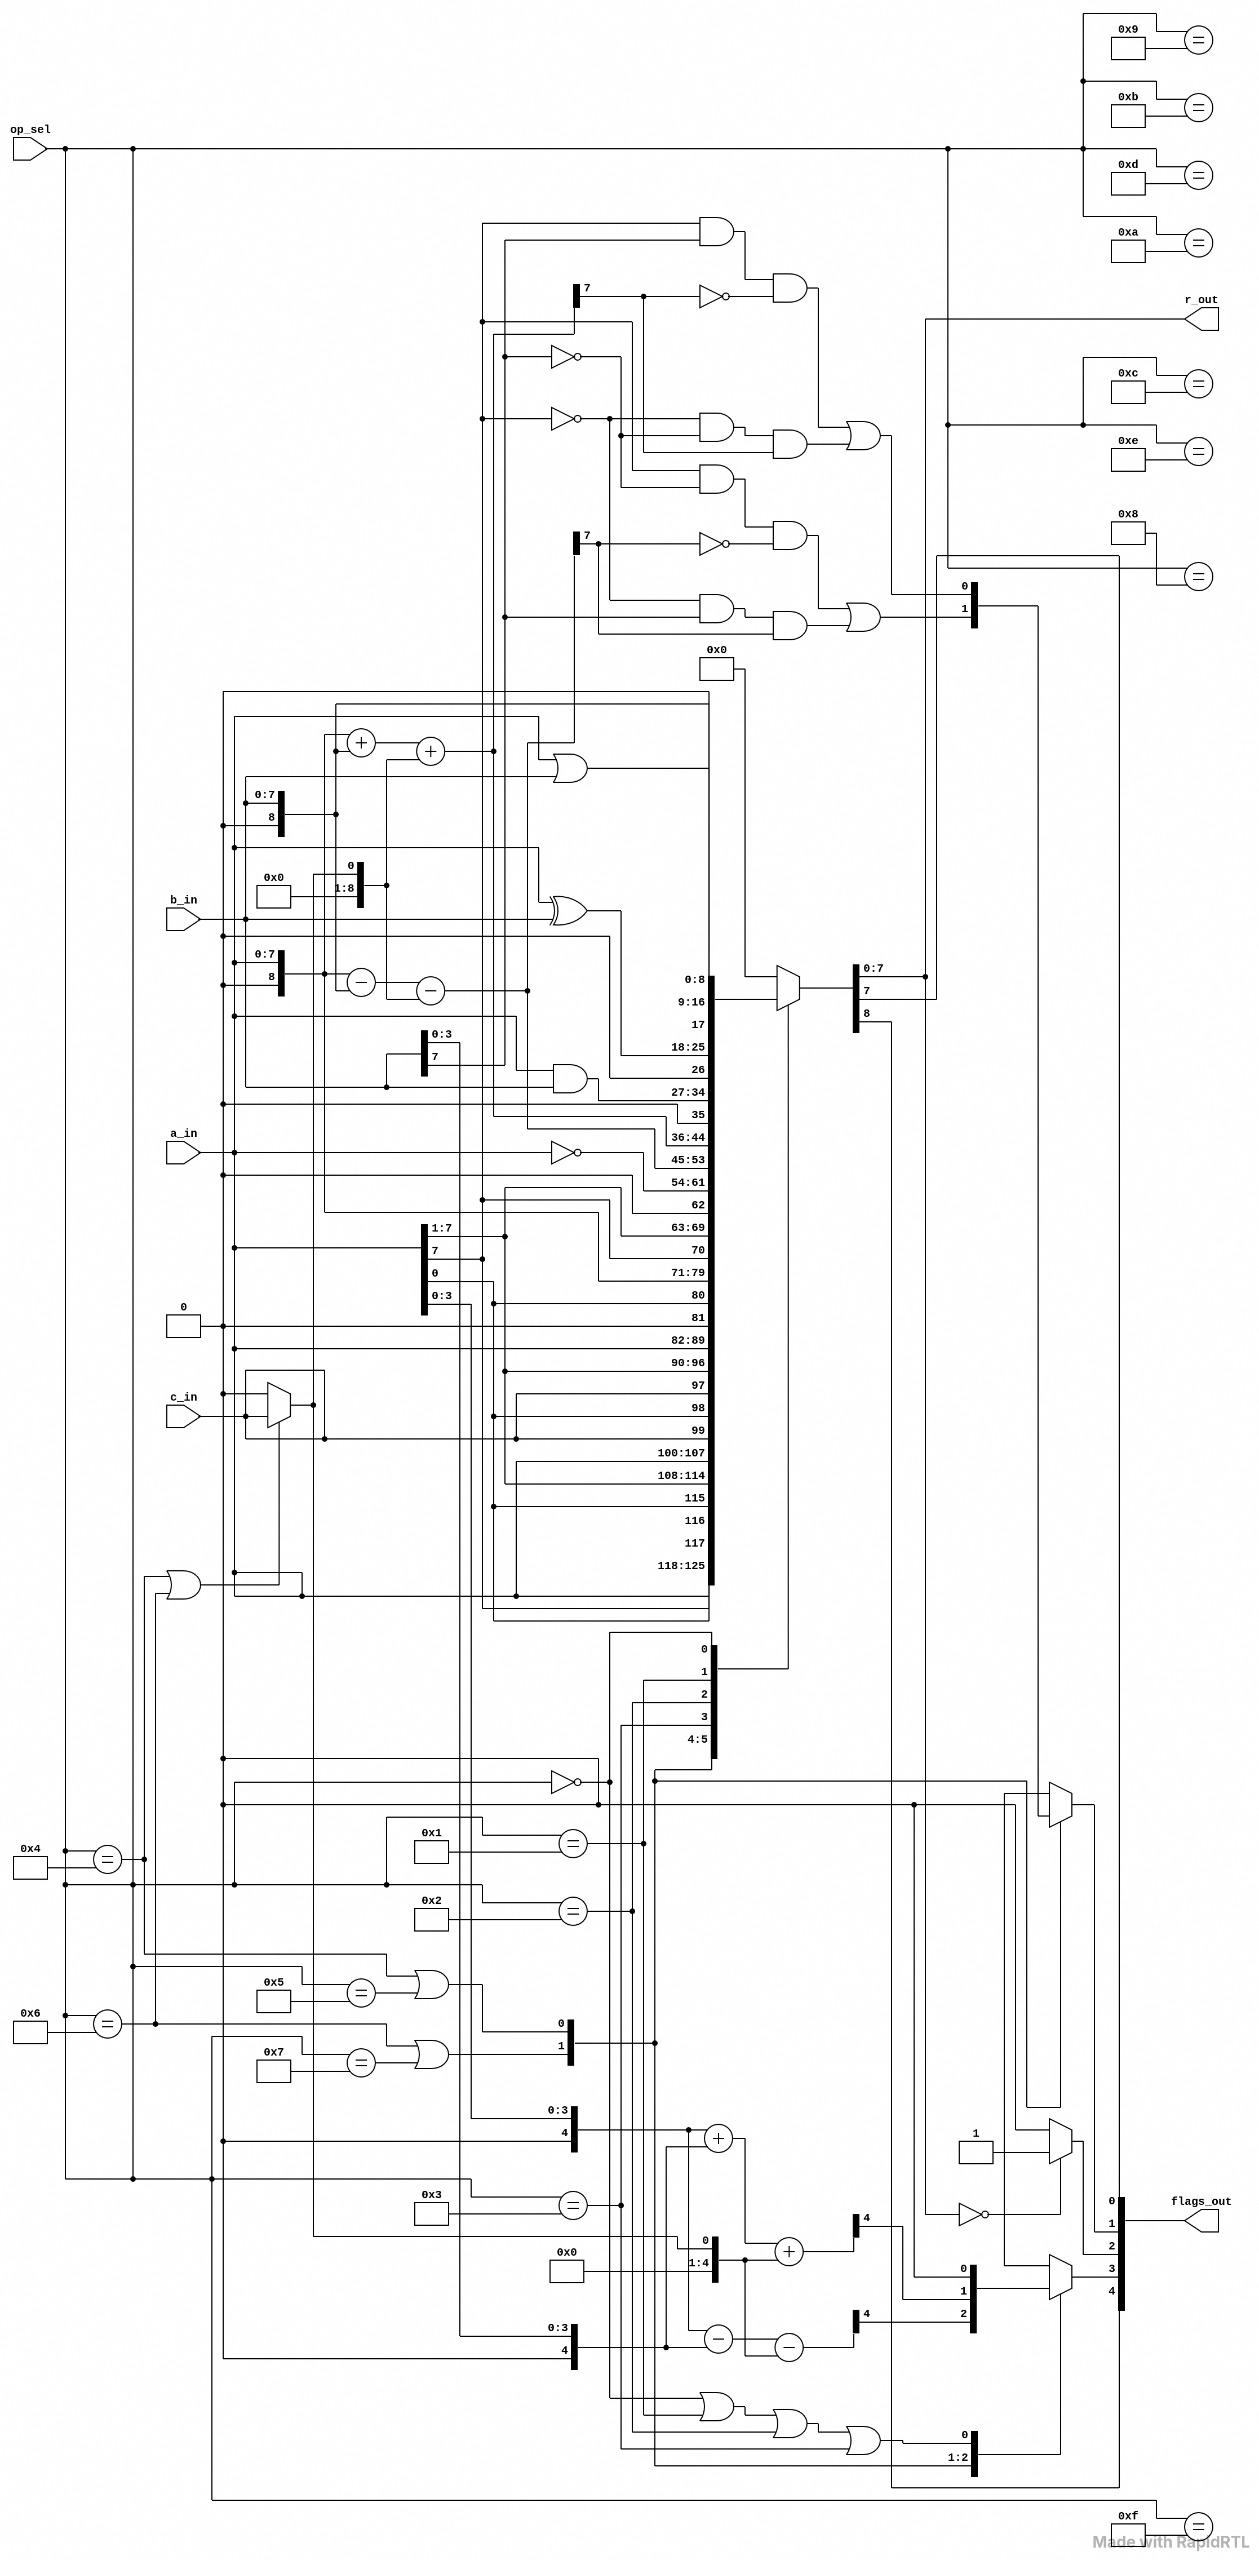
\includegraphics[
    width=0.95\textwidth,
    height=0.75\textheight,
    keepaspectratio
  ]{image/Portas-Logicas-Verticais.jpeg}
  \fonte{Elaborado a partir do site RapidRTL, utilizado como base o coigo fonte (alu.vhd).}
\end{figure}

\newpage
\section{Decisões de projeto}

\begin{itemize}
  \item \textbf{Subtração por soma}: usa-se a identidade da Equação~\ref{eq:sub}. O bit \texttt{op\_sel(1)} distingue subtração ($\texttt{1}$) de soma ($\texttt{0}$) e \texttt{op\_sel(0)} indica se o carry de entrada é usado (\texttt{0}). O carry de entrada do somador é
  \[
    c_{add} = \overline{s}\cdot\overline{op_0}\cdot c_{in} \;+\; s\cdot\overline{\overline{op_0}\cdot c_{in}},
  \]
  em que $s$ = \texttt{op\_sel(1)}.
  \item \textbf{Borrow}: em subtrações, C e H são o carry do somador invertido (XOR com $s$). Equação~\ref{eq:sub}.
  \item \textbf{Overflow}: calculado pela Equação~\ref{eq:ovf} usando o operando efetivo $b_{op}$.
  \item \textbf{\textit{Don't care}}: nas operações em que a especificação não define H ou V, essas flags são fixadas em `0', o que evita lógica desnecessária e saídas indefinidas na simulação.
\end{itemize}

\section{Código-fonte}

O Código~\ref{lst:alu} apresenta a entidade e a arquitetura completas, com comentários.

\lstinputlisting[
  style=vhdl,
  caption={Descrição VHDL da ALU (\texttt{alu.vhd}).},
  label={lst:alu},
  basicstyle=\ttfamily\scriptsize,
  breaklines=true,
  frame=single,
  extendedchars=true,
  literate={á}{{\'a}}1 {ã}{{\~a}}1 {ç}{{\c c}}1
            {é}{{\'e}}1 {ê}{{\^e}}1 {ó}{{\'o}}1 {õ}{{\~o}}1
]{vhdl/alu.vhd}
\vspace{-0.3cm}
\fonte{Autoria propria.}
%-----------------------------------------------------
\chapter{Simulação e Resultados}
\label{cap:simulacao}

\section{Metodologia}

A simulação funcional foi feita no Quartus II 9.1sp2 com o editor de formas de onda (arquivo \texttt{.vwf}). Como o circuito é combinacional, cada vetor de teste define \texttt{a\_in}, \texttt{b\_in}, \texttt{c\_in} e \texttt{op\_sel}, e o resultado é conferido após o atraso de propagação.

Os casos de teste cobrem: (i) todas as 16 operações; (ii) os seis exemplos de ADD da especificação, assim como 6 outros exemplos para as demais 15 operações; (iii) situações-limite das flags, como carry, \textit{half carry}, overflow positivo e negativo, resultado zero e resultado negativo; e (iv) o uso de \texttt{c\_in} em ADDC, SUBC, RRC e RLC.


\section{Casos de teste e resultados esperados}

As Tabelas ~\ref{tab:testes-PASS-B} a ~\ref{tab:testes-RL} lista os casos usados. Os traços indicam flags \textit{don't care} (fixadas em `0' no projeto).

\begin{longtable}{c c c c c c c c c c}
\caption{Casos de teste da operação PASS\_B.}
\label{tab:testes-PASS-B}\\
\hline
Caso & \texttt{a\_in} & \texttt{b\_in} & \texttt{c\_in} & \texttt{r\_out} & C & H & Z & V & N \\ \hline
\endfirsthead
\hline
Caso & \texttt{a\_in} & \texttt{b\_in} & \texttt{c\_in} & \texttt{r\_out} & C & H & Z & V & N \\ \hline
\endhead
1 & FF & A5 & 0 & A5 & 0 & 0 & 0 & {\footnotesize--} & 1 \\
2 & FF & 00 & 1 & 00 & 0 & 0 & 1 & {\footnotesize--} & 0 \\
3 & 12 & 7F & 0 & 7F & 0 & 0 & 0 & {\footnotesize--} & 0 \\
4 & 55 & 80 & 1 & 80 & 0 & 0 & 0 & {\footnotesize--} & 1 \\
5 & 00 & FF & 0 & FF & 0 & 0 & 0 & {\footnotesize--} & 1 \\
6 & F0 & 01 & 1 & 01 & 0 & 0 & 0 & {\footnotesize--} & 0 \\
\hline
\end{longtable}
\vspace{-0.5cm}
\fonte{Autoria propria.}

\begin{longtable}{c c c c c c c c c c}
\caption{Casos de teste da operação OR.}
\label{tab:testes-OR}\\
\hline
Caso & \texttt{a\_in} & \texttt{b\_in} & \texttt{c\_in} & \texttt{r\_out} & C & H & Z & V & N \\ \hline
\endfirsthead
\hline
Caso & \texttt{a\_in} & \texttt{b\_in} & \texttt{c\_in} & \texttt{r\_out} & C & H & Z & V & N \\ \hline
\endhead
7 & 00 & 00 & 0 & 00 & 0 & 0 & 1 & {\footnotesize--} & 0 \\
8 & F0 & 0F & 0 & FF & 0 & 0 & 0 & {\footnotesize--} & 1 \\
9 & A5 & 00 & 0 & A5 & 0 & 0 & 0 & {\footnotesize--} & 1 \\
10 & 80 & 01 & 0 & 81 & 0 & 0 & 0 & {\footnotesize--} & 1 \\
11 & 55 & AA & 0 & FF & 0 & 0 & 0 & {\footnotesize--} & 1 \\
12 & 0F & 30 & 1 & 3F & 0 & 0 & 0 & {\footnotesize--} & 0 \\
\hline
\end{longtable}
\vspace{-0.5cm}
\fonte{Autoria propria.}

\begin{longtable}{c c c c c c c c c c}
\caption{Casos de teste da operação XOR.}
\label{tab:testes-XOR}\\
\hline
Caso & \texttt{a\_in} & \texttt{b\_in} & \texttt{c\_in} & \texttt{r\_out} & C & H & Z & V & N \\ \hline
\endfirsthead
\hline
Caso & \texttt{a\_in} & \texttt{b\_in} & \texttt{c\_in} & \texttt{r\_out} & C & H & Z & V & N \\ \hline
\endhead
13 & FF & FF & 0 & 00 & 0 & 0 & 1 & {\footnotesize--} & 0 \\
14 & AA & 55 & 0 & FF & 0 & 0 & 0 & {\footnotesize--} & 1 \\
15 & F0 & 0F & 0 & FF & 0 & 0 & 0 & {\footnotesize--} & 1 \\
16 & B5 & 4C & 0 & F9 & 0 & 0 & 0 & {\footnotesize--} & 1 \\
17 & 00 & 00 & 0 & 00 & 0 & 0 & 1 & {\footnotesize--} & 0 \\
18 & 80 & 80 & 1 & 00 & 0 & 0 & 1 & {\footnotesize--} & 0 \\
\hline
\end{longtable}
\vspace{-0.5cm}
\fonte{Autoria propria.}

\begin{longtable}{c c c c c c c c c c}
\caption{Casos de teste da operação AND.}
\label{tab:testes-AND}\\
\hline
Caso & \texttt{a\_in} & \texttt{b\_in} & \texttt{c\_in} & \texttt{r\_out} & C & H & Z & V & N \\ \hline
\endfirsthead
\hline
Caso & \texttt{a\_in} & \texttt{b\_in} & \texttt{c\_in} & \texttt{r\_out} & C & H & Z & V & N \\ \hline
\endhead
19 & 0F & F0 & 0 & 00 & 0 & 0 & 1 & {\footnotesize--} & 0 \\
20 & FF & FF & 0 & FF & 0 & 0 & 0 & {\footnotesize--} & 1 \\
21 & F0 & 3C & 0 & 30 & 0 & 0 & 0 & {\footnotesize--} & 0 \\
22 & B5 & 4C & 0 & 04 & 0 & 0 & 0 & {\footnotesize--} & 0 \\
23 & 80 & FF & 0 & 80 & 0 & 0 & 0 & {\footnotesize--} & 1 \\
24 & 55 & AA & 1 & 00 & 0 & 0 & 1 & {\footnotesize--} & 0 \\
\hline
\end{longtable}
\vspace{-0.5cm}
\fonte{Autoria propria.}

\begin{longtable}{c c c c c c c c c c}
\caption{Casos de teste da operação ADDC.}
\label{tab:testes-ADDC}\\
\hline
Caso & \texttt{a\_in} & \texttt{b\_in} & \texttt{c\_in} & \texttt{r\_out} & C & H & Z & V & N \\ \hline
\endfirsthead
\hline
Caso & \texttt{a\_in} & \texttt{b\_in} & \texttt{c\_in} & \texttt{r\_out} & C & H & Z & V & N \\ \hline
\endhead
25 & 0F & 01 & 0 & 10 & 0 & 1 & 0 & 0 & 0 \\
26 & 0F & 01 & 1 & 11 & 0 & 1 & 0 & 0 & 0 \\
27 & FF & 00 & 1 & 00 & 1 & 1 & 1 & 0 & 0 \\
28 & 7F & 00 & 1 & 80 & 0 & 1 & 0 & 1 & 1 \\
29 & FF & FF & 1 & FF & 1 & 1 & 0 & 0 & 1 \\
30 & 80 & 80 & 1 & 01 & 1 & 0 & 0 & 1 & 0 \\
\hline
\end{longtable}
\vspace{-0.5cm}
\fonte{Autoria propria.}

\begin{longtable}{c c c c c c c c c c}
\caption{Casos de teste da operação ADD.}
\label{tab:testes-ADD}\\
\hline
Caso & \texttt{a\_in} & \texttt{b\_in} & \texttt{c\_in} & \texttt{r\_out} & C & H & Z & V & N \\ \hline
\endfirsthead
\hline
Caso & \texttt{a\_in} & \texttt{b\_in} & \texttt{c\_in} & \texttt{r\_out} & C & H & Z & V & N \\ \hline
\endhead
31 & 37 & 10 & 0 & 47 & 0 & 0 & 0 & 0 & 0 \\
32 & 37 & 19 & 0 & 50 & 0 & 1 & 0 & 0 & 0 \\
33 & 77 & 70 & 0 & E7 & 0 & 0 & 0 & 1 & 1 \\
34 & 77 & 89 & 0 & 00 & 1 & 1 & 1 & 0 & 0 \\
35 & 80 & 80 & 0 & 00 & 1 & 0 & 1 & 1 & 0 \\
36 & C7 & D0 & 0 & 97 & 1 & 0 & 0 & 0 & 1 \\
\hline
\end{longtable}
\vspace{-0.5cm}
\fonte{Autoria propria.}

\begin{longtable}{c c c c c c c c c c}
\caption{Casos de teste da operação SUBC.}
\label{tab:testes-SUBC}\\
\hline
Caso & \texttt{a\_in} & \texttt{b\_in} & \texttt{c\_in} & \texttt{r\_out} & C & H & Z & V & N \\ \hline
\endfirsthead
\hline
Caso & \texttt{a\_in} & \texttt{b\_in} & \texttt{c\_in} & \texttt{r\_out} & C & H & Z & V & N \\ \hline
\endhead
37 & 10 & 0F & 1 & 00 & 0 & 1 & 1 & 0 & 0 \\
38 & 10 & 0F & 0 & 01 & 0 & 1 & 0 & 0 & 0 \\
39 & 00 & 00 & 1 & FF & 1 & 1 & 0 & 0 & 1 \\
40 & 80 & 00 & 1 & 7F & 0 & 1 & 0 & 1 & 0 \\
41 & 50 & B0 & 0 & A0 & 1 & 0 & 0 & 1 & 1 \\
42 & 05 & 05 & 0 & 00 & 0 & 0 & 1 & 0 & 0 \\
\hline
\end{longtable}
\vspace{-0.5cm}
\fonte{Autoria propria.}

\begin{longtable}{c c c c c c c c c c}
\caption{Casos de teste da operação SUB.}
\label{tab:testes-SUB}\\
\hline
Caso & \texttt{a\_in} & \texttt{b\_in} & \texttt{c\_in} & \texttt{r\_out} & C & H & Z & V & N \\ \hline
\endfirsthead
\hline
Caso & \texttt{a\_in} & \texttt{b\_in} & \texttt{c\_in} & \texttt{r\_out} & C & H & Z & V & N \\ \hline
\endhead
43 & 10 & 01 & 0 & 0F & 0 & 1 & 0 & 0 & 0 \\
44 & 05 & 05 & 0 & 00 & 0 & 0 & 1 & 0 & 0 \\
45 & 00 & 01 & 0 & FF & 1 & 1 & 0 & 0 & 1 \\
46 & 80 & 01 & 0 & 7F & 0 & 1 & 0 & 1 & 0 \\
47 & 50 & B0 & 0 & A0 & 1 & 0 & 0 & 1 & 1 \\
48 & 10 & 01 & 1 & 0F & 0 & 1 & 0 & 0 & 0 \\
\hline
\end{longtable}
\vspace{-0.5cm}
\fonte{Autoria propria.}

\begin{longtable}{c c c c c c c c c c}
\caption{Casos de teste da operação NOT.}
\label{tab:testes-NOT}\\
\hline
Caso & \texttt{a\_in} & \texttt{b\_in} & \texttt{c\_in} & \texttt{r\_out} & C & H & Z & V & N \\ \hline
\endfirsthead
\hline
Caso & \texttt{a\_in} & \texttt{b\_in} & \texttt{c\_in} & \texttt{r\_out} & C & H & Z & V & N \\ \hline
\endhead
49 & 0F & 00 & 0 & F0 & 0 & {\footnotesize--} & 0 & {\footnotesize--} & 1 \\
50 & FF & 00 & 0 & 00 & 0 & {\footnotesize--} & 1 & {\footnotesize--} & 0 \\
51 & 00 & 00 & 0 & FF & 0 & {\footnotesize--} & 0 & {\footnotesize--} & 1 \\
52 & AA & 55 & 1 & 55 & 0 & {\footnotesize--} & 0 & {\footnotesize--} & 0 \\
53 & 80 & 00 & 0 & 7F & 0 & {\footnotesize--} & 0 & {\footnotesize--} & 0 \\
54 & 7F & 00 & 0 & 80 & 0 & {\footnotesize--} & 0 & {\footnotesize--} & 1 \\
\hline
\end{longtable}
\vspace{-0.5cm}
\fonte{Autoria propria.}

\begin{longtable}{c c c c c c c c c c}
\caption{Casos de teste da operação SRA.}
\label{tab:testes-SRA}\\
\hline
Caso & \texttt{a\_in} & \texttt{b\_in} & \texttt{c\_in} & \texttt{r\_out} & C & H & Z & V & N \\ \hline
\endfirsthead
\hline
Caso & \texttt{a\_in} & \texttt{b\_in} & \texttt{c\_in} & \texttt{r\_out} & C & H & Z & V & N \\ \hline
\endhead
55 & 81 & 00 & 0 & C0 & 1 & {\footnotesize--} & 0 & {\footnotesize--} & 1 \\
56 & 01 & 00 & 0 & 00 & 1 & {\footnotesize--} & 1 & {\footnotesize--} & 0 \\
57 & 7E & 00 & 0 & 3F & 0 & {\footnotesize--} & 0 & {\footnotesize--} & 0 \\
58 & 80 & 00 & 0 & C0 & 0 & {\footnotesize--} & 0 & {\footnotesize--} & 1 \\
59 & FF & 00 & 0 & FF & 1 & {\footnotesize--} & 0 & {\footnotesize--} & 1 \\
60 & 00 & 00 & 1 & 00 & 0 & {\footnotesize--} & 1 & {\footnotesize--} & 0 \\
\hline
\end{longtable}
\vspace{-0.5cm}
\fonte{Autoria propria.}

\begin{longtable}{c c c c c c c c c c}
\caption{Casos de teste da operação SRL.}
\label{tab:testes-SRL}\\
\hline
Caso & \texttt{a\_in} & \texttt{b\_in} & \texttt{c\_in} & \texttt{r\_out} & C & H & Z & V & N \\ \hline
\endfirsthead
\hline
Caso & \texttt{a\_in} & \texttt{b\_in} & \texttt{c\_in} & \texttt{r\_out} & C & H & Z & V & N \\ \hline
\endhead
61 & 81 & 00 & 0 & 40 & 1 & {\footnotesize--} & 0 & {\footnotesize--} & 0 \\
62 & 01 & 00 & 0 & 00 & 1 & {\footnotesize--} & 1 & {\footnotesize--} & 0 \\
63 & FE & 00 & 0 & 7F & 0 & {\footnotesize--} & 0 & {\footnotesize--} & 0 \\
64 & FF & 00 & 0 & 7F & 1 & {\footnotesize--} & 0 & {\footnotesize--} & 0 \\
65 & 80 & 00 & 0 & 40 & 0 & {\footnotesize--} & 0 & {\footnotesize--} & 0 \\
66 & 00 & 00 & 1 & 00 & 0 & {\footnotesize--} & 1 & {\footnotesize--} & 0 \\
\hline
\end{longtable}
\vspace{-0.5cm}
\fonte{Autoria propria.}

\begin{longtable}{c c c c c c c c c c}
\caption{Casos de teste da operação SLL.}
\label{tab:testes-SLL}\\
\hline
Caso & \texttt{a\_in} & \texttt{b\_in} & \texttt{c\_in} & \texttt{r\_out} & C & H & Z & V & N \\ \hline
\endfirsthead
\hline
Caso & \texttt{a\_in} & \texttt{b\_in} & \texttt{c\_in} & \texttt{r\_out} & C & H & Z & V & N \\ \hline
\endhead
67 & 81 & 00 & 0 & 02 & 1 & {\footnotesize--} & 0 & {\footnotesize--} & 0 \\
68 & 40 & 00 & 0 & 80 & 0 & {\footnotesize--} & 0 & {\footnotesize--} & 1 \\
69 & 01 & 00 & 0 & 02 & 0 & {\footnotesize--} & 0 & {\footnotesize--} & 0 \\
70 & FF & 00 & 0 & FE & 1 & {\footnotesize--} & 0 & {\footnotesize--} & 1 \\
71 & 80 & 00 & 0 & 00 & 1 & {\footnotesize--} & 1 & {\footnotesize--} & 0 \\
72 & 00 & 00 & 1 & 00 & 0 & {\footnotesize--} & 1 & {\footnotesize--} & 0 \\
\hline
\end{longtable}
\vspace{-0.5cm}
\fonte{Autoria propria.}

\begin{longtable}{c c c c c c c c c c}
\caption{Casos de teste da operação RRC.}
\label{tab:testes-RRC}\\
\hline
Caso & \texttt{a\_in} & \texttt{b\_in} & \texttt{c\_in} & \texttt{r\_out} & C & H & Z & V & N \\ \hline
\endfirsthead
\hline
Caso & \texttt{a\_in} & \texttt{b\_in} & \texttt{c\_in} & \texttt{r\_out} & C & H & Z & V & N \\ \hline
\endhead
73 & 01 & 00 & 1 & 80 & 1 & {\footnotesize--} & 0 & {\footnotesize--} & 1 \\
74 & 01 & 00 & 0 & 00 & 1 & {\footnotesize--} & 1 & {\footnotesize--} & 0 \\
75 & 00 & 00 & 1 & 80 & 0 & {\footnotesize--} & 0 & {\footnotesize--} & 1 \\
76 & FF & 00 & 0 & 7F & 1 & {\footnotesize--} & 0 & {\footnotesize--} & 0 \\
77 & 80 & 00 & 1 & C0 & 0 & {\footnotesize--} & 0 & {\footnotesize--} & 1 \\
78 & A5 & 00 & 0 & 52 & 1 & {\footnotesize--} & 0 & {\footnotesize--} & 0 \\
\hline
\end{longtable}
\vspace{-0.5cm}
\fonte{Autoria propria.}

\begin{longtable}{c c c c c c c c c c}
\caption{Casos de teste da operação RLC.}
\label{tab:testes-RLC}\\
\hline
Caso & \texttt{a\_in} & \texttt{b\_in} & \texttt{c\_in} & \texttt{r\_out} & C & H & Z & V & N \\ \hline
\endfirsthead
\hline
Caso & \texttt{a\_in} & \texttt{b\_in} & \texttt{c\_in} & \texttt{r\_out} & C & H & Z & V & N \\ \hline
\endhead
79 & 80 & 00 & 1 & 01 & 1 & {\footnotesize--} & 0 & {\footnotesize--} & 0 \\
80 & 80 & 00 & 0 & 00 & 1 & {\footnotesize--} & 1 & {\footnotesize--} & 0 \\
81 & 00 & 00 & 1 & 01 & 0 & {\footnotesize--} & 0 & {\footnotesize--} & 0 \\
82 & FF & 00 & 0 & FE & 1 & {\footnotesize--} & 0 & {\footnotesize--} & 1 \\
83 & 01 & 00 & 1 & 03 & 0 & {\footnotesize--} & 0 & {\footnotesize--} & 0 \\
84 & 5A & 00 & 0 & B4 & 0 & {\footnotesize--} & 0 & {\footnotesize--} & 1 \\
\hline
\end{longtable}
\vspace{-0.5cm}
\fonte{Autoria propria.}

\begin{longtable}{c c c c c c c c c c}
\caption{Casos de teste da operação RR.}
\label{tab:testes-RR}\\
\hline
Caso & \texttt{a\_in} & \texttt{b\_in} & \texttt{c\_in} & \texttt{r\_out} & C & H & Z & V & N \\ \hline
\endfirsthead
\hline
Caso & \texttt{a\_in} & \texttt{b\_in} & \texttt{c\_in} & \texttt{r\_out} & C & H & Z & V & N \\ \hline
\endhead
85 & 01 & 00 & 0 & 80 & 1 & {\footnotesize--} & 0 & {\footnotesize--} & 1 \\
86 & 02 & 00 & 0 & 01 & 0 & {\footnotesize--} & 0 & {\footnotesize--} & 0 \\
87 & 80 & 00 & 1 & 40 & 0 & {\footnotesize--} & 0 & {\footnotesize--} & 0 \\
88 & FF & 00 & 0 & FF & 1 & {\footnotesize--} & 0 & {\footnotesize--} & 1 \\
89 & A5 & 00 & 0 & D2 & 1 & {\footnotesize--} & 0 & {\footnotesize--} & 1 \\
90 & 00 & 00 & 1 & 00 & 0 & {\footnotesize--} & 1 & {\footnotesize--} & 0 \\
\hline
\end{longtable}
\vspace{-0.5cm}
\fonte{Autoria propria.}

\begin{longtable}{c c c c c c c c c c}
\caption{Casos de teste da operação RL.}
\label{tab:testes-RL}\\
\hline
Caso & \texttt{a\_in} & \texttt{b\_in} & \texttt{c\_in} & \texttt{r\_out} & C & H & Z & V & N \\ \hline
\endfirsthead
\hline
Caso & \texttt{a\_in} & \texttt{b\_in} & \texttt{c\_in} & \texttt{r\_out} & C & H & Z & V & N \\ \hline
\endhead
91 & 80 & 00 & 0 & 01 & 1 & {\footnotesize--} & 0 & {\footnotesize--} & 0 \\
92 & 40 & 00 & 0 & 80 & 0 & {\footnotesize--} & 0 & {\footnotesize--} & 1 \\
93 & 01 & 00 & 1 & 02 & 0 & {\footnotesize--} & 0 & {\footnotesize--} & 0 \\
94 & FF & 00 & 0 & FF & 1 & {\footnotesize--} & 0 & {\footnotesize--} & 1 \\
95 & A5 & 00 & 0 & 4B & 1 & {\footnotesize--} & 0 & {\footnotesize--} & 0 \\
96 & 00 & 00 & 1 & 00 & 0 & {\footnotesize--} & 1 & {\footnotesize--} & 0 \\
\hline
\end{longtable}
\vspace{-0.5cm}
\fonte{Autoria propria.}


\clearpage
\section{Formas de ondas}

\begin{figure}[!htb]
  \centering
  \caption{Simulação funcional da operação PASS\_B (\texttt{op\_sel = 0000}).}
  \label{fig:sim-pass-b}
  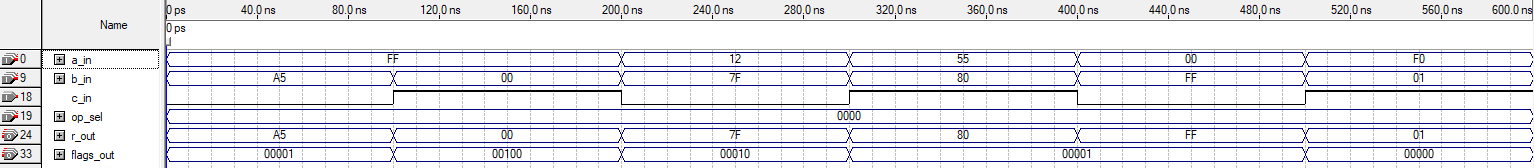
\includegraphics[width=\textwidth]{image/PASS_B.png}
  \fonte{Autoria propria (Quartus II 9.1sp2).}
\end{figure}

\begin{figure}[!htb]
  \centering
  \caption{Simulação funcional da operação OR (\texttt{op\_sel = 0001}).}
  \label{fig:sim-or}
  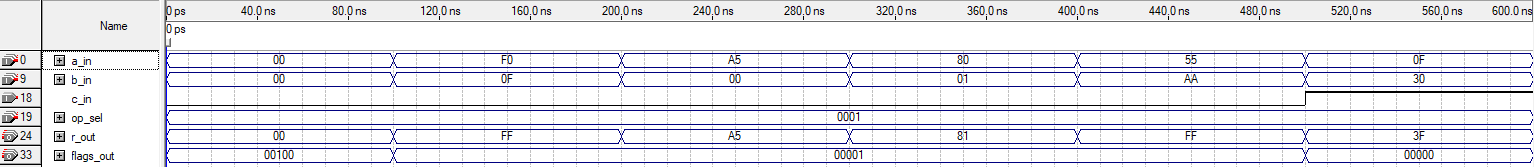
\includegraphics[width=\textwidth]{image/OR.png}
  \fonte{Autoria propria (Quartus II 9.1sp2).}
\end{figure}

\begin{figure}[!htb]
  \centering
  \caption{Simulação funcional da operação XOR (\texttt{op\_sel = 0010}).}
  \label{fig:sim-xor}
  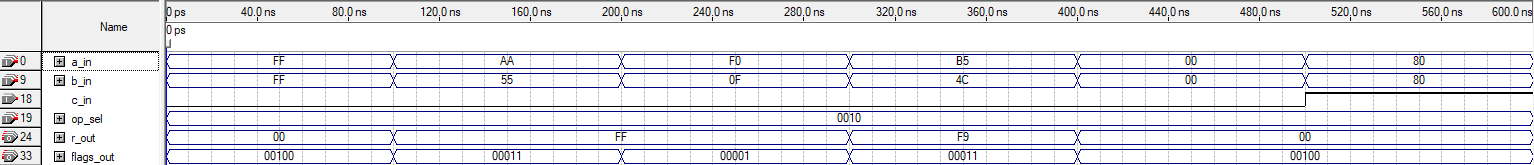
\includegraphics[width=\textwidth]{image/XOR.png}
  \fonte{Autoria propria (Quartus II 9.1sp2).}
\end{figure}

\begin{figure}[!htb]
  \centering
  \caption{Simulação funcional da operação AND (\texttt{op\_sel = 0011}).}
  \label{fig:sim-and}
  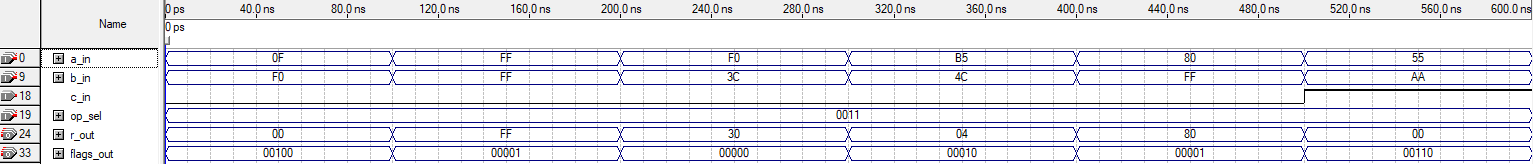
\includegraphics[width=\textwidth]{image/AND.png}
  \fonte{Autoria propria (Quartus II 9.1sp2).}
\end{figure}

\begin{figure}[!htb]
  \centering
  \caption{Simulação funcional da operação ADDC (\texttt{op\_sel = 0100}).}
  \label{fig:sim-addc}
  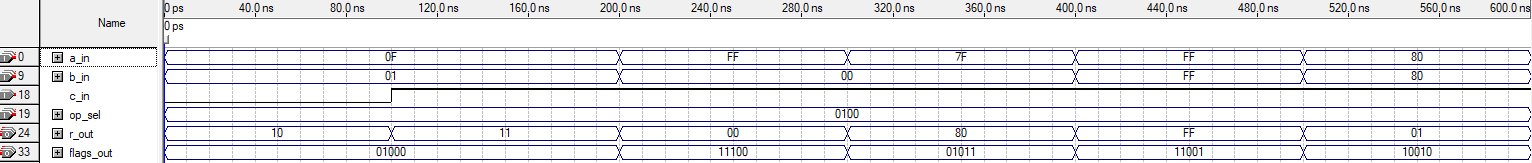
\includegraphics[width=\textwidth]{image/ADDC.png}
  \fonte{Autoria propria (Quartus II 9.1sp2).}
\end{figure}

\begin{figure}[!htb]
  \centering
  \caption{Simulação funcional da operação ADD (\texttt{op\_sel = 0101}).}
  \label{fig:sim-add}
  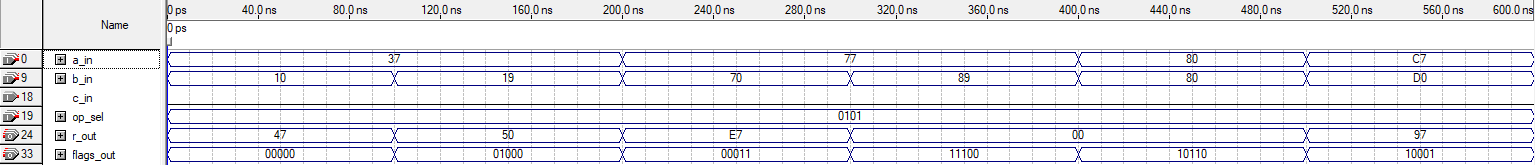
\includegraphics[width=\textwidth]{image/ADD.png}
  \fonte{Autoria propria (Quartus II 9.1sp2).}
\end{figure}

\begin{figure}[!htb]
  \centering
  \caption{Simulação funcional da operação SUBC (\texttt{op\_sel = 0110}).}
  \label{fig:sim-subc}
  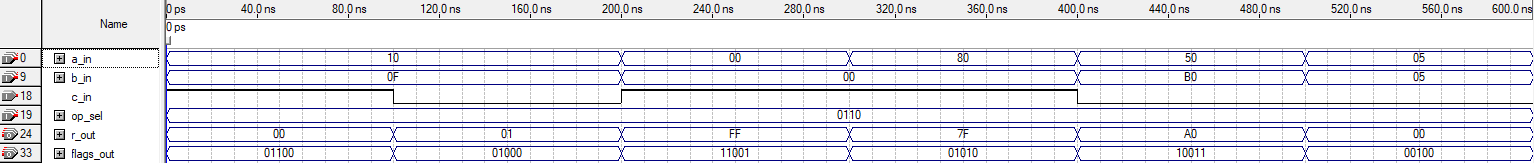
\includegraphics[width=\textwidth]{image/SUBC.png}
  \fonte{Autoria propria (Quartus II 9.1sp2).}
\end{figure}

\begin{figure}[!htb]
  \centering
  \caption{Simulação funcional da operação SUB (\texttt{op\_sel = 0111}).}
  \label{fig:sim-sub}
  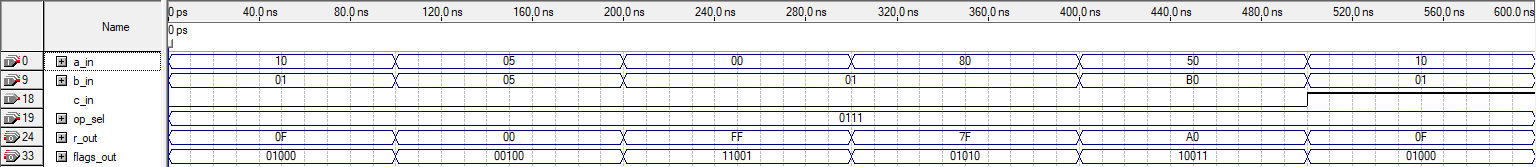
\includegraphics[width=\textwidth]{image/SUB.png}
  \fonte{Autoria propria (Quartus II 9.1sp2).}
\end{figure}

\begin{figure}[!htb]
  \centering
  \caption{Simulação funcional da operação NOT (\texttt{op\_sel = 1000}).}
  \label{fig:sim-not}
  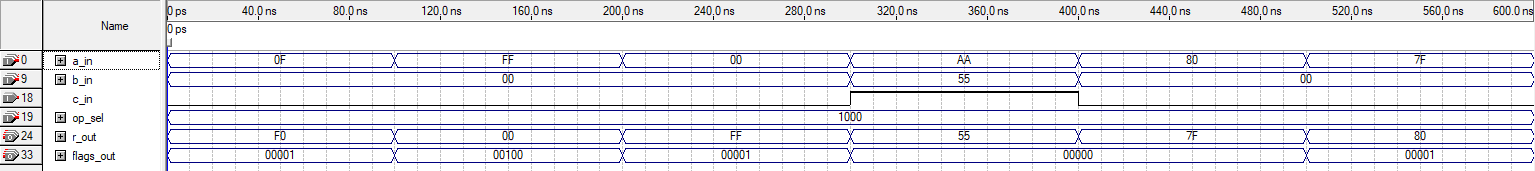
\includegraphics[width=\textwidth]{image/NOT.png}
  \fonte{Autoria propria (Quartus II 9.1sp2).}
\end{figure}

\begin{figure}[!htb]
  \centering
  \caption{Simulação funcional da operação SRA (\texttt{op\_sel = 1001}).}
  \label{fig:sim-sra}
  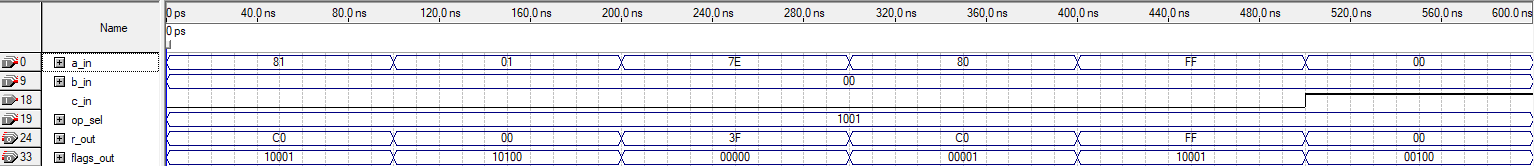
\includegraphics[width=\textwidth]{image/SRA.png}
  \fonte{Autoria propria (Quartus II 9.1sp2).}
\end{figure}

\begin{figure}[!htb]
  \centering
  \caption{Simulação funcional da operação SRL (\texttt{op\_sel = 1010}).}
  \label{fig:sim-srl}
  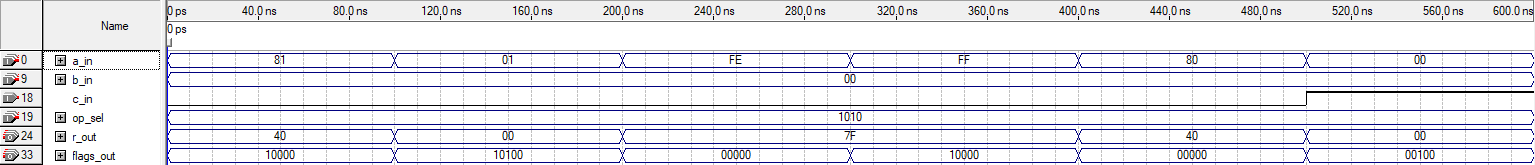
\includegraphics[width=\textwidth]{image/SRL.png}
  \fonte{Autoria propria (Quartus II 9.1sp2).}
\end{figure}

\begin{figure}[!htb]
  \centering
  \caption{Simulação funcional da operação SLL (\texttt{op\_sel = 1011}).}
  \label{fig:sim-sll}
  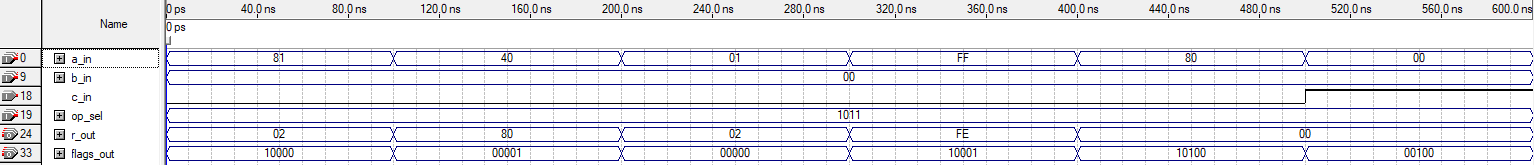
\includegraphics[width=\textwidth]{image/SLL.png}
  \fonte{Autoria propria (Quartus II 9.1sp2).}
\end{figure}

\begin{figure}[!htb]
  \centering
  \caption{Simulação funcional da operação RRC (\texttt{op\_sel = 1100}).}
  \label{fig:sim-rrc}
  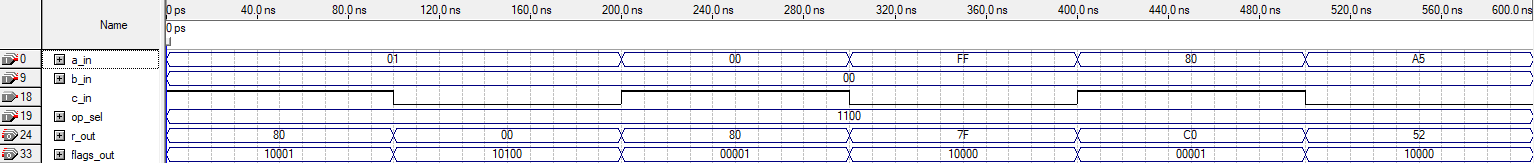
\includegraphics[width=\textwidth]{image/RRC.png}
  \fonte{Autoria propria (Quartus II 9.1sp2).}
\end{figure}

\begin{figure}[!htb]
  \centering
  \caption{Simulação funcional da operação RLC (\texttt{op\_sel = 1101}).}
  \label{fig:sim-rlc}
  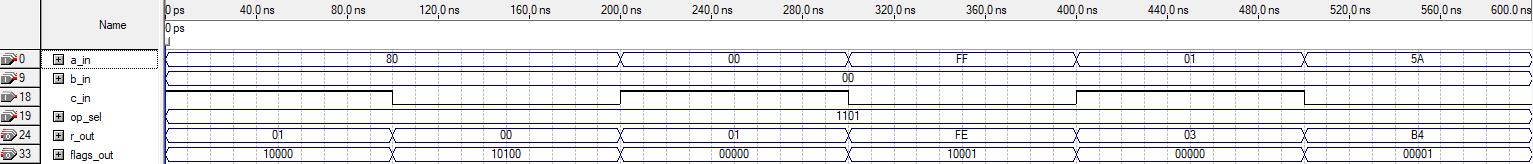
\includegraphics[width=\textwidth]{image/RLC.png}
  \fonte{Autoria propria (Quartus II 9.1sp2).}
\end{figure}

\begin{figure}[!htb]
  \centering
  \caption{Simulação funcional da operação RR (\texttt{op\_sel = 1110}).}
  \label{fig:sim-rr}
  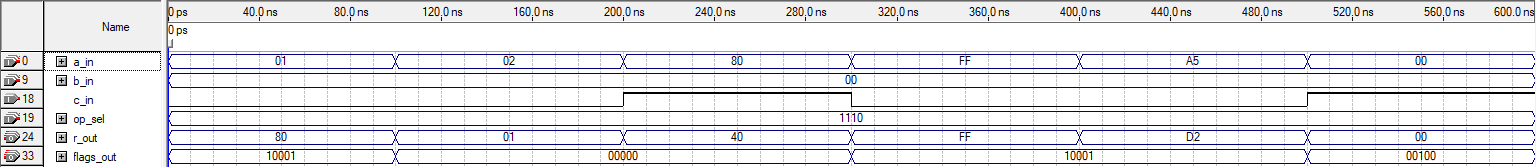
\includegraphics[width=\textwidth]{image/RR.png}
  \fonte{Autoria propria (Quartus II 9.1sp2).}
\end{figure}

\begin{figure}[!htb]
  \centering
  \caption{Simulação funcional da operação RL (\texttt{op\_sel = 1111}).}
  \label{fig:sim-rl}
  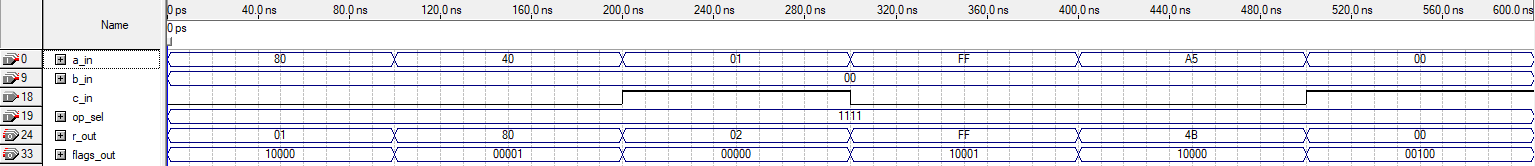
\includegraphics[width=\textwidth]{image/RL.png}
  \fonte{Autoria propria (Quartus II 9.1sp2).}
\end{figure}

\clearpage
\section{Análise dos resultados}

Os resultados foram analisados a partir dos 96 casos apresentados nas tabelas
individuais de cada operação e das formas de onda obtidas no Quartus II. Em
todos os casos, foram comparados o valor de \texttt{r\_out} e o estado das
flags C, H, Z, V e N. Essa comparação é importante porque uma operação pode
produzir o resultado numérico correto e, ainda assim, apresentar erro em uma
das flags.

\subsection{Operações lógicas}

As operações \texttt{PASS\_B}, \texttt{OR}, \texttt{XOR} e \texttt{AND}
apresentaram o comportamento esperado para todas as combinações testadas. Em
\texttt{PASS\_B}, o resultado acompanha diretamente \texttt{b\_in},
independentemente do valor de \texttt{a\_in} e de \texttt{c\_in}. Nas demais
operações, cada bit do resultado corresponde à aplicação da operação lógica
entre os bits de mesma posição dos operandos.

Nessas quatro operações, C e H permanecem em zero, pois não existe propagação
de carry ou borrow. A flag V também é tratada como ``don't care'' pela
especificação e foi mantida em zero na implementação. As flags Z e N foram
geradas a partir do resultado selecionado: Z é ativada somente quando
\texttt{r\_out} é igual a zero, enquanto N reproduz o bit mais significativo
do resultado. Os casos com resultados \texttt{00} e \texttt{FF} confirmam,
respectivamente, o funcionamento das flags Z e N.

\subsection{Operações de soma}

As operações \texttt{ADDC} e \texttt{ADD} confirmaram o funcionamento do
caminho aritmético compartilhado. Em \texttt{ADDC}, o valor de
\texttt{c\_in} participa da soma; em \texttt{ADD}, ele é ignorado e o carry
inicial é zero. A diferença pode ser observada nos casos em que os operandos
são iguais, mas o carry de entrada varia, como em
$0F + 01 + 0 = 10$ e $0F + 01 + 1 = 11$.

Os seis exemplos de \texttt{ADD} da especificação também foram reproduzidos.
O caso $37h + 10h = 47h$ não produz flags de exceção; $37h + 19h = 50h$
produz \textit{half carry}; e $77h + 70h = E7h$ apresenta overflow e
resultado negativo. No caso $77h + 89h = 00h$, ocorre simultaneamente carry,
\textit{half carry} e zero. Já $80h + 80h = 00h$ demonstra a ocorrência de
carry e overflow com resultado zero, enquanto $C7h + D0h = 97h$ produz carry
sem overflow. Esses casos mostram que carry e overflow representam condições
diferentes: o primeiro está relacionado ao transporte além do oitavo bit, e o
segundo à interpretação com sinal.

\subsection{Operações de subtração}

Os resultados de \texttt{SUBC} e \texttt{SUB} confirmam a implementação da
subtração por complemento de dois. O operando B é invertido e o carry inicial
é ajustado para que a soma produza a diferença desejada. Em \texttt{SUBC},
\texttt{c\_in} é incluído como empréstimo; em \texttt{SUB}, a operação é feita
sem empréstimo inicial.

Nas subtrações, C e H representam borrow, conforme a convenção adotada no
projeto. Por exemplo, $10h - 20h = F0h$ gera borrow e resultado negativo.
Também é possível observar a diferença entre borrow e overflow no caso
$80h - 01h = 7Fh$: o resultado aritmético excede o intervalo representável
com sinal, portanto V é ativada, embora o resultado binário seja positivo.
Nos casos em que os operandos são iguais, o resultado é zero, Z é ativada e
as flags de borrow permanecem inativas.

\subsection{Deslocamentos e rotações}

Nas operações \texttt{SRA}, \texttt{SRL} e \texttt{SLL}, o bit removido da
palavra é copiado para C. A operação \texttt{SRA} preserva o bit de sinal ao
preencher a posição mais significativa, enquanto \texttt{SRL} preenche essa
posição com zero. Em \texttt{SLL}, o bit menos significativo recebe zero e o
bit mais significativo deslocado é utilizado para atualizar C.

Os resultados confirmam, por exemplo, que \texttt{81h} deslocado
aritmeticamente à direita produz \texttt{C0h}, preservando o bit de sinal, ao
passo que o deslocamento lógico produz \texttt{40h}. Em todas essas operações,
H e V não são relevantes e permanecem fixadas em zero, conforme definido na
especificação.

Nas rotações com carry, \texttt{RRC} e \texttt{RLC}, o valor de
\texttt{c\_in} é inserido na palavra durante a rotação. Em \texttt{RRC}, o
bit menos significativo deslocado ocupa a posição de C e o carry de entrada
entra no bit mais significativo. Em \texttt{RLC}, ocorre o processo inverso.
Os casos com \texttt{c\_in} igual a zero e a um confirmam que essa entrada
não é apenas uma flag de controle, mas participa efetivamente do resultado.

Nas rotações \texttt{RR} e \texttt{RL}, não há carry de entrada: o bit
expulso retorna pela extremidade oposta da palavra. Assim, a rotação de
\texttt{01h} para a direita produz \texttt{80h}, enquanto a rotação de
\texttt{80h} para a esquerda produz \texttt{01h}. Esses casos também
confirmam que C recebe o bit que foi expulso.

\subsection{Avaliação geral das flags}

As flags Z e N foram consistentes em todas as classes de operação. Z foi
ativada para resultados \texttt{00h}, inclusive quando o valor zero foi
obtido por uma soma, subtração, operação lógica ou deslocamento. N acompanhou
corretamente o bit 7 de \texttt{r\_out}, permanecendo ativa para resultados
como \texttt{80h}, \texttt{A5h}, \texttt{C0h} e \texttt{FFh}.

As flags C, H e V foram avaliadas de acordo com a natureza da operação. C e H
foram utilizados nas operações aritméticas, C também registrou o bit expulso
nos deslocamentos e rotações, e V foi utilizada para indicar overflow com
sinal nas somas e subtrações. Nas operações em que a especificação não define
uma dessas flags, o valor zero evita estados indefinidos e torna a forma de
onda mais simples de interpretar.

De modo geral, a comparação entre as tabelas de resultados esperados e as
formas de onda confirma a correção funcional da ALU para as 16 operações
implementadas. Os testes também verificam as situações de limite mais
relevantes, incluindo carry, borrow, \textit{half carry}, overflow, zero,
resultado negativo e o uso do carry de entrada.

%-----------------------------------------------------
\chapter{Conclusão}
\label{cap:conclusao}

Foi desenvolvida e verificada uma ALU combinacional de 8 bits com 16 operações e 5 flags, descrita em VHDL com código exclusivamente concorrente e interfaces \break \texttt{std\_logic}/\texttt{std\_logic\_vector}, como exigido. Compartilhar um único somador/subtrator entre ADDC, ADD, SUBC e SUB, com inversão do operando B e do carry de entrada, reduziu a lógica e simplificou o cálculo das flags de carry/borrow, \textit{half carry/borrow} e overflow.

Os resultados da simulação concordaram com os valores esperados em todos os casos, inclusive nos seis exemplos de ADD da especificação. Como trabalho futuro, a ALU pode ser integrada a um caminho de dados com registradores de flags, ou ter o desempenho (atraso de propagação e uso de elementos lógicos) comparado entre diferentes arquiteturas de somador.

%-----------------------------------------------------

% ELEMENTOS PÓS-TEXTUAIS ------------------------------------------------------

\postextual

\pagestyle{plain}

%----------------------------------------------------
% Referências bibliográficas
%----------------------------------------------------

\printbibliography[heading=bibintoc,title={Referências}]

%-----------------------------------------------------
% Glossário 
%-----------------------------------------------------
% Consulte o manual da classe abntex2 para orientações sobre o glossário.

%\glossary

%-----------------------------------------------------
% Apêndices 
%-----------------------------------------------------
% Inicia os apêndices
%---

\begin{apendicesenv}
\chapter{Arquivos do projeto}
\label{ap:arquivos}

O projeto foi organizado para separar a descrição do circuito, os arquivos de
simulação, os dados de verificação e os arquivos usados na documentação. A
estrutura entregue deve conter os seguintes itens:

\begin{description}
  \item[\texttt{vhdl/alu.vhd}] descrição VHDL da ALU, apresentada no
    Código~\ref{lst:alu}. O arquivo contém a entidade, a arquitetura
    combinacional, o caminho aritmético compartilhado, a seleção das operações
    e a geração das flags.
  \item[\texttt{image/}] formas de onda exportadas da simulação, uma para
    cada operação, na mesma ordem apresentada no Capítulo~\ref{cap:simulacao}:
    \texttt{PASS\_B.png}, \texttt{OR.png}, \texttt{XOR.png},
    \texttt{AND.png}, \texttt{ADDC.png}, \texttt{ADD.png},
    \texttt{SUBC.png}, \texttt{SUB.png}, \texttt{NOT.png},
    \texttt{SRA.png}, \texttt{SRL.png}, \texttt{SLL.png},
    \texttt{RRC.png}, \texttt{RLC.png}, \texttt{RR.png} e
    \texttt{RL.png}.
  \item[\texttt{tabelas/resultados\_esperados.md}] consolidação dos casos de
    teste, com entradas, resultados e flags esperadas para as 16 operações.
  \item[\texttt{tabelas/TP1\_<operação>\_tabela.md}] tabelas individuais
    dos resultados esperados por operação.
  \item[\texttt{capitulos/tabela\_testes.tex}] versão LaTeX das tabelas de
    teste, usada no Capítulo~\ref{cap:simulacao}.
  \item[\texttt{Dissertação.tex}], \texttt{config/} e \texttt{capitulos/}
    arquivos principais da documentação, incluindo o preâmbulo, as
    configurações, os capítulos e este apêndice.
\end{description}

\end{apendicesenv}

%--- 

%-----------------------------------------------------
% Anexos (não utilizados)
%-----------------------------------------------------

% Este relatório não possui anexos.

%-----------------------------------------------------
% INDICE REMISSIVO
%-----------------------------------------------------

% Este relatório não utiliza índice remissivo.
% \input{capitulos/indiceremiss.tex}

%-----------------------------------------------------
\end{document}
